\documentclass[xcolor=dvipsnames,10pt]{beamer}

\usepackage{tikz}
\usetikzlibrary{arrows}
\usepackage{verbatim}
\usepackage[active,tightpage]{preview}
\setlength\PreviewBorder{5pt}%

\mode<presentation>

%\usepackage[hidelinks]{hyperref}
\usepackage{beamerthemesplit}
\usepackage[UKenglish]{babel}
%\usepackage{cite}
\usepackage{listings}
\usepackage{latexsym}
\usepackage[utf8]{inputenc}
\usepackage{multirow}
\usepackage{listings}
\usepackage{color}
\usepackage{amsmath,amsthm,amssymb}
\usepackage[noend]{algpseudocode}
\usepackage[ruled,noline,linesnumbered, slide]{algorithm2e}
\usepackage{pgf}
\usepackage{tikz}
\usetikzlibrary{automata,arrows,decorations.pathreplacing}
\usetikzlibrary{positioning}
\usepackage{epstopdf}

%%Notation:

%%vectors
\renewcommand{\vec}[1]{\boldsymbol{#1}}
%%sets
\newcommand{\set}[1]{\mathcal{#1}}
%%matrixes
\newcommand{\mat}[1]{#1}
%%norm
\newcommand{\norm}[1]{\left\Vert #1 \right\Vert}
%%defeq
\newcommand{\defeq}{\triangleq}
%%
\newcommand{\net}[1]{\mathrm{#1}}
%% pair<x,y>
\newcommand{\pair}[2]{\langle#1,#2\rangle}

%%%%%%%%%%%%%%%%%%%%%%%%%%%%%%%%%%%%
\usepackage{sansmathaccent}
\pdfmapfile{+sansmathaccent.map}

\definecolor{dkgreen}{rgb}{0,0.6,0}
\definecolor{mauve}{rgb}{0.58,0,0.82}

\graphicspath{ {./images/} }


\usecolortheme[named=MidnightBlue]{structure}

%Warsaw Dresden Singapore Copenhagen Madrid AnnArbor
\usetheme{Warsaw}
\setbeamercovered{transparent}
\setbeamercolor{lowercolor}{fg=white , bg=MidnightBlue}
\setbeamertemplate{blocks}[rounded][shadow=true]
\setbeamertemplate{items}[default]
\setbeamertemplate{navigation symbols}{}

\def\hilite<#1>{%
\temporal<#1>{\color{lightgray}}{\color{black}}%
{\color{black}}}

\usetitlepagetemplate{
  \begin{center}

    \begin{beamerboxesrounded}[lower=lowercolor, shadow=true]{}
     \begin{center}
    \normalsize{Recurrent neural networks}
     \end{center}
    \end{beamerboxesrounded}
    \vspace{3em}
    Giulio Galvan
    
  \end{center}
}

\title[Recurrent neural network]{}
\author{Giulio Galvan}
\date{\today}

\newcommand*\oldmacro{}%
\let\oldmacro\insertshorttitle%
\renewcommand*\insertshorttitle{%
  \oldmacro\hfill%
  \insertframenumber\,/\,\inserttotalframenumber}

\begin{document}

\frame{\titlepage}
\section{Introduction}
 
\begin{frame}{The model}
	
\begin{block}{RNN}
	Given an input sequences $\{\vec{u}\}_{t=1,...,T}$, with $ \vec{u}_t \in \mathbb{R}^p$, the output sequence of a RNN $\{\vec{y}\}_{t=1,...,T}$, with $\vec{y}_t \in \mathbb{R}^o$,  is defined by the following:
\begin{align}
		&\vec{y}^t \defeq F(W^{out}\cdot\vec{a}^t + \vec{b}^{out})\\
		&\vec{a}^t \defeq W^{rec}\cdot\vec{h}^{t-1}+W^{in}\cdot\vec{u}^t+\vec{b}^{rec}\\
		&\vec{h}^t \defeq  \sigma(\vec{a}^t) \\
		&\vec{h}^0 \defeq \overrightarrow{0},
\end{align}
where $\sigma(\cdot):\mathbb{R}\rightarrow\mathbb{R}$ is a non linear function applied element-wise called activation function.
\end{block}
\end{frame}

\begin{frame}{The optimization problem}
Given a dataset $D$:
\begin{equation}
D\defeq\{\{\overline{\vec{u}}^{(i)}\}_{t=1,...,T}, \overline{\vec{u}}^{(i)}_t \in \mathbb{R}^p, \{\overline{\vec{y}}^{(i)}\}_{t=1,...,T}, \overline{\vec{y}}^{(i)}_t \in \mathbb{R}^o;  i=1,...,N\}
\end{equation}
we define a loss function $L_D:\mathbb{R}^N \rightarrow \mathbb{R}_{\geq 0}$ over $D$  as
\begin{equation}
L_D(\vec{x})\defeq\frac{1}{N}\sum_{i=1}^N \sum_{t=1}^T L_t(\overline{\vec{y}}_t^{(i)},\vec{y}_t^{(i)}(\vec{x})),
\end{equation}
where $L_t(\cdot, \cdot)$ is an arbitrary loss function for the time step $t$.
The problem is \begin{equation}
\min_{\vec{x}\in \mathbb{R}^N} L_D(\vec{x})
\end{equation}
\end{frame}

\begin{frame}{Stochastic gradient descent (SGD)}
SGD is the standard framework in most of the applications.
\begin{algorithm}[H]
	\KwData{\\
		\Indp
		$D=\{\pair{\vec{u}^{(i)}}{\vec{y}^{(i)}}\}$: training set\\
		$\vec{x}_0$: candidate solution \\
		$m$: size of each minibatch\\
	}
	
	\KwResult{\\
		\Indp $\vec{x}$: solution
	}
	\BlankLine
	
	$\vec{x} \gets \vec{x}_0$\\
	\While{stop criterion}{
		
		$I$ $\gets$ select $m$ training example $\in D$  \\
		$\alpha \gets$ compute learning rate \\
		$\vec{x} \gets \vec{x} - \alpha \sum_{ i\in I}\nabla_{\vec{x}} L(\vec{x}; \pair{\vec{u}^{(i)}}{\vec{y}^{(i)}})$\\
	}
	\caption{Stochastic gradient descent}
	\label{algo:sgd}
\end{algorithm}	
\end{frame}
\section{The vanishing gradient problem}
\begin{frame}{A pathological problem example}


An input sequence:

\vspace{1em}

\begin{tabular}{|c|c|c|c|c|c|c|c|c|c}
	\hline  marker & 0&  1&  0&  $\hdots$& 0 & 1 & 0 & 0  \\ 
	  value & 0.3&  \textbf{0.7}&  0.1&  $\hdots$& 0.2& \textbf{0.4} & 0.6& 0.9  \\ 
	\hline 
\end{tabular}

\vspace{1em}
The predicted output should be the sum of the two one marked positions (1.1). 
\pause
\vspace{1em}
\begin{block}{Why is this a difficult problem?}
	\pause
	Because of it's long time dependencies.
\end{block}

\end{frame}

\begin{frame}{Unfolding}
	\tikzstyle{rnn_style}=[->,shorten >=1pt,auto,node distance=1.5cm,
	thick,
	neuron/.style={circle,fill=white!50,draw,minimum size=0.7cm,font=\sffamily\Large\bfseries},
	missing/.style={circle,fill=white!50,draw=none,minimum size=0.7cm,font=\sffamily\Huge\bfseries},
	label/.style={node distance=1.2cm,rectangle,fill=white!50,draw=none,minimum size=0.7cm,font=\sffamily\normalsize},
	layer/.style={rectangle,fill=white!50,draw,minimum width=4cm,font=\sffamily\normalsize},
	loopStyle/.style={in=120,out=60, distance=2.5cm},]
	

		
	\begin{figure}[h!]
		\centering
		\resizebox{8cm}{!}{
		\begin{tikzpicture}[rnn_style]
		
		%t=0
		\node[layer] (hl1) {Hidden layer t=0};
		
		\node[neuron]    (x0)[below left=0.3cm and 1cm of hl1]       {};
		\node[label]    (u0)[left of=x0]   {$\vec{u}_1$};
		
		
		
		\node[neuron] (o0) [above right=0.3cm and 1cm of hl1] {};
		\node[label]    (y0)[right of=o0]   {$\vec{y}_1$};
		
		%t=1
		\node[layer] (hl2)[above of=hl1,node distance=2.5cm] {Hidden layer t=1};
		
		\node[neuron]    (x1)[below left=0.3cm and 1cm of hl2]      {};
		\node[label]    (u1)[left of=x1]   {$\vec{u}_2$};
		
		
		\node[neuron] (o1) [above right=0.3cm and 1cm of hl2] {};
		\node[label]    (y1)[right of=o1]   {$\vec{y}_2$};
		
		%dots
		\node[label,font=\sffamily\Huge\bfseries] (hld)[above of=hl2,node distance=2cm] {$\hdots$};
		
		%t=T
		\node[layer] (hlT)[above of=hld,node distance=2cm] {Hidden layer t=T};
		
		\node[neuron]    (xT)[below left=0.3cm and 1cm of hlT]      {};
		\node[label]    (uT)[left of=xT]   {$\vec{u}_T$};
		
		
		\node[neuron] (oT) [above right=0.3cm and 1cm of  hlT] {};
		\node[label]    (yT)[right of=oT]   {$\vec{y}_T$};
		
		
		%biases
		\node[neuron](b) [right of=y1,node distance=1.4cm] {};
		\node[label] (b_l) [above of=b,node distance=0.7cm] {bias=1};
		
		
		\path[->] (x0) edge [bend right] node[]{$W^{in}$}   (hl1)
		(u0) edge []   (x0)
		(o0) edge []   (y0)
		(x1) edge [bend right] node[]{$W^{in}$} (hl2)
		(u1) edge []   (x1)
		(o1) edge []   (y1)
		(xT) edge [bend right] node[]{$W^{in}$} (hlT)
		(uT) edge []   (xT)
		(oT) edge []   (yT)
		
		
		(hl1) edge [bend left]  node[]{$W^{out}$} (o0)
		(hl2) edge [bend left]  node[]{$W^{out}$} (o1)
		(hlT) edge [bend left]  node[]{$W^{out}$} (oT)
		
		(b)  edge [bend left,dotted,in = 90]  node[]{$b^{out}$} (o0)
		(b)  edge [bend left, dotted, in = 90,out=80]  node[]{$b^{rec}$} (hl1)
		(b)  edge [bend left, dotted]  node[]{$b^{rec}$} (hl2)
		(b)  edge [bend left,dotted]  node[]{$b^{out}$} (o1)
		(b)  edge [bend left, dotted,in = 200]  node[]{$b^{rec}$} (hlT)
		(b)  edge [bend left,dotted,in =200]  node[]{$b^{out}$} (oT)
		(hl1) edge [] node[]{$W^{rec} $} (hl2)
		(hl2) edge [] node[]{$W^{rec} $} (hld)
		(hld) edge [] node[]{$W^{rec} $} (hlT);
		
		\end{tikzpicture}
	}
		\caption{Unfolding of a $\net{RNN}$}
		\label{rnn_unfolding}
	\end{figure}
\end{frame}

\begin{frame}{Understanding the gradient structure}
	Simply applying the chain rule it's easy to see that
	\begin{equation}
		\nabla L(\vec{x}) = \sum_{t=1}^T \nabla L_{|t}(\vec{x}),
	\end{equation}
	where $\nabla L_{|t}$ is ...
\end{frame}

\begin{frame}{Vanishing gradient: an upper bound}
	\begin{equation}
	\frac{\partial \vec{a}^t}{\partial \vec{a}^k} = \prod_{i=t-1}^{k}  diag(\sigma'(\vec{a}^i)) \cdot \mat{W}^{rec}.
	\label{eq:temporalComponent}
	\end{equation}
	
	Taking the singular value decomposition of $\mat{W}^{rec}$:
	\begin{equation}
	\mat{W}^{rec} =  \mat{S}\cdot\mat{D}\cdot\mat{V}^T
	\end{equation}
	where $\mat{S},\mat{V}^T$ are squared orthogonal matrices and $\mat{D}\defeq diag(\mu_1, \mu_2,...,\mu_r)$ is the diagonal matrix containing the singular values of $\mat{W}^{rec}$.
	Hence:
	\begin{equation}
	\frac{\partial \vec{a}^t}{\partial \vec{a}^k} = \prod_{i=t-1}^{k}  diag(\sigma'(\vec{a}^i)) \cdot \mat{S}\cdot \mat{D} \cdot \mat{V}^T
	\end{equation}
	\end{frame}
	\begin{frame}
			Since $\mat{U}$ and $\mat{V}$ are orthogonal matrix, hence $$\norm{\mat{U}}_2=\norm{\mat{V}^T}_2 = 1,$$ and $$\norm{diag(\lambda_1, \lambda_2,...,\lambda_r)}_2 \leq \lambda_{max},$$ we get
			\begin{align}
			\norm{\frac{\partial \vec{a}^t}{\partial \vec{a}^k}}_2 &= \norm{ (\prod_{i=t-1}^{k} diag(\sigma'(\vec{a}^i)) \cdot \mat{S}\cdot \mat{D} \cdot \mat{V}^T)}_2\\
			&\leq (\sigma'_{max} \cdot \mu_{max})^{t-k-1}
			\end{align}
	\end{frame}



\begin{frame}{Temporal gradient norms: an illustration}
\begin{figure}
	\centering
	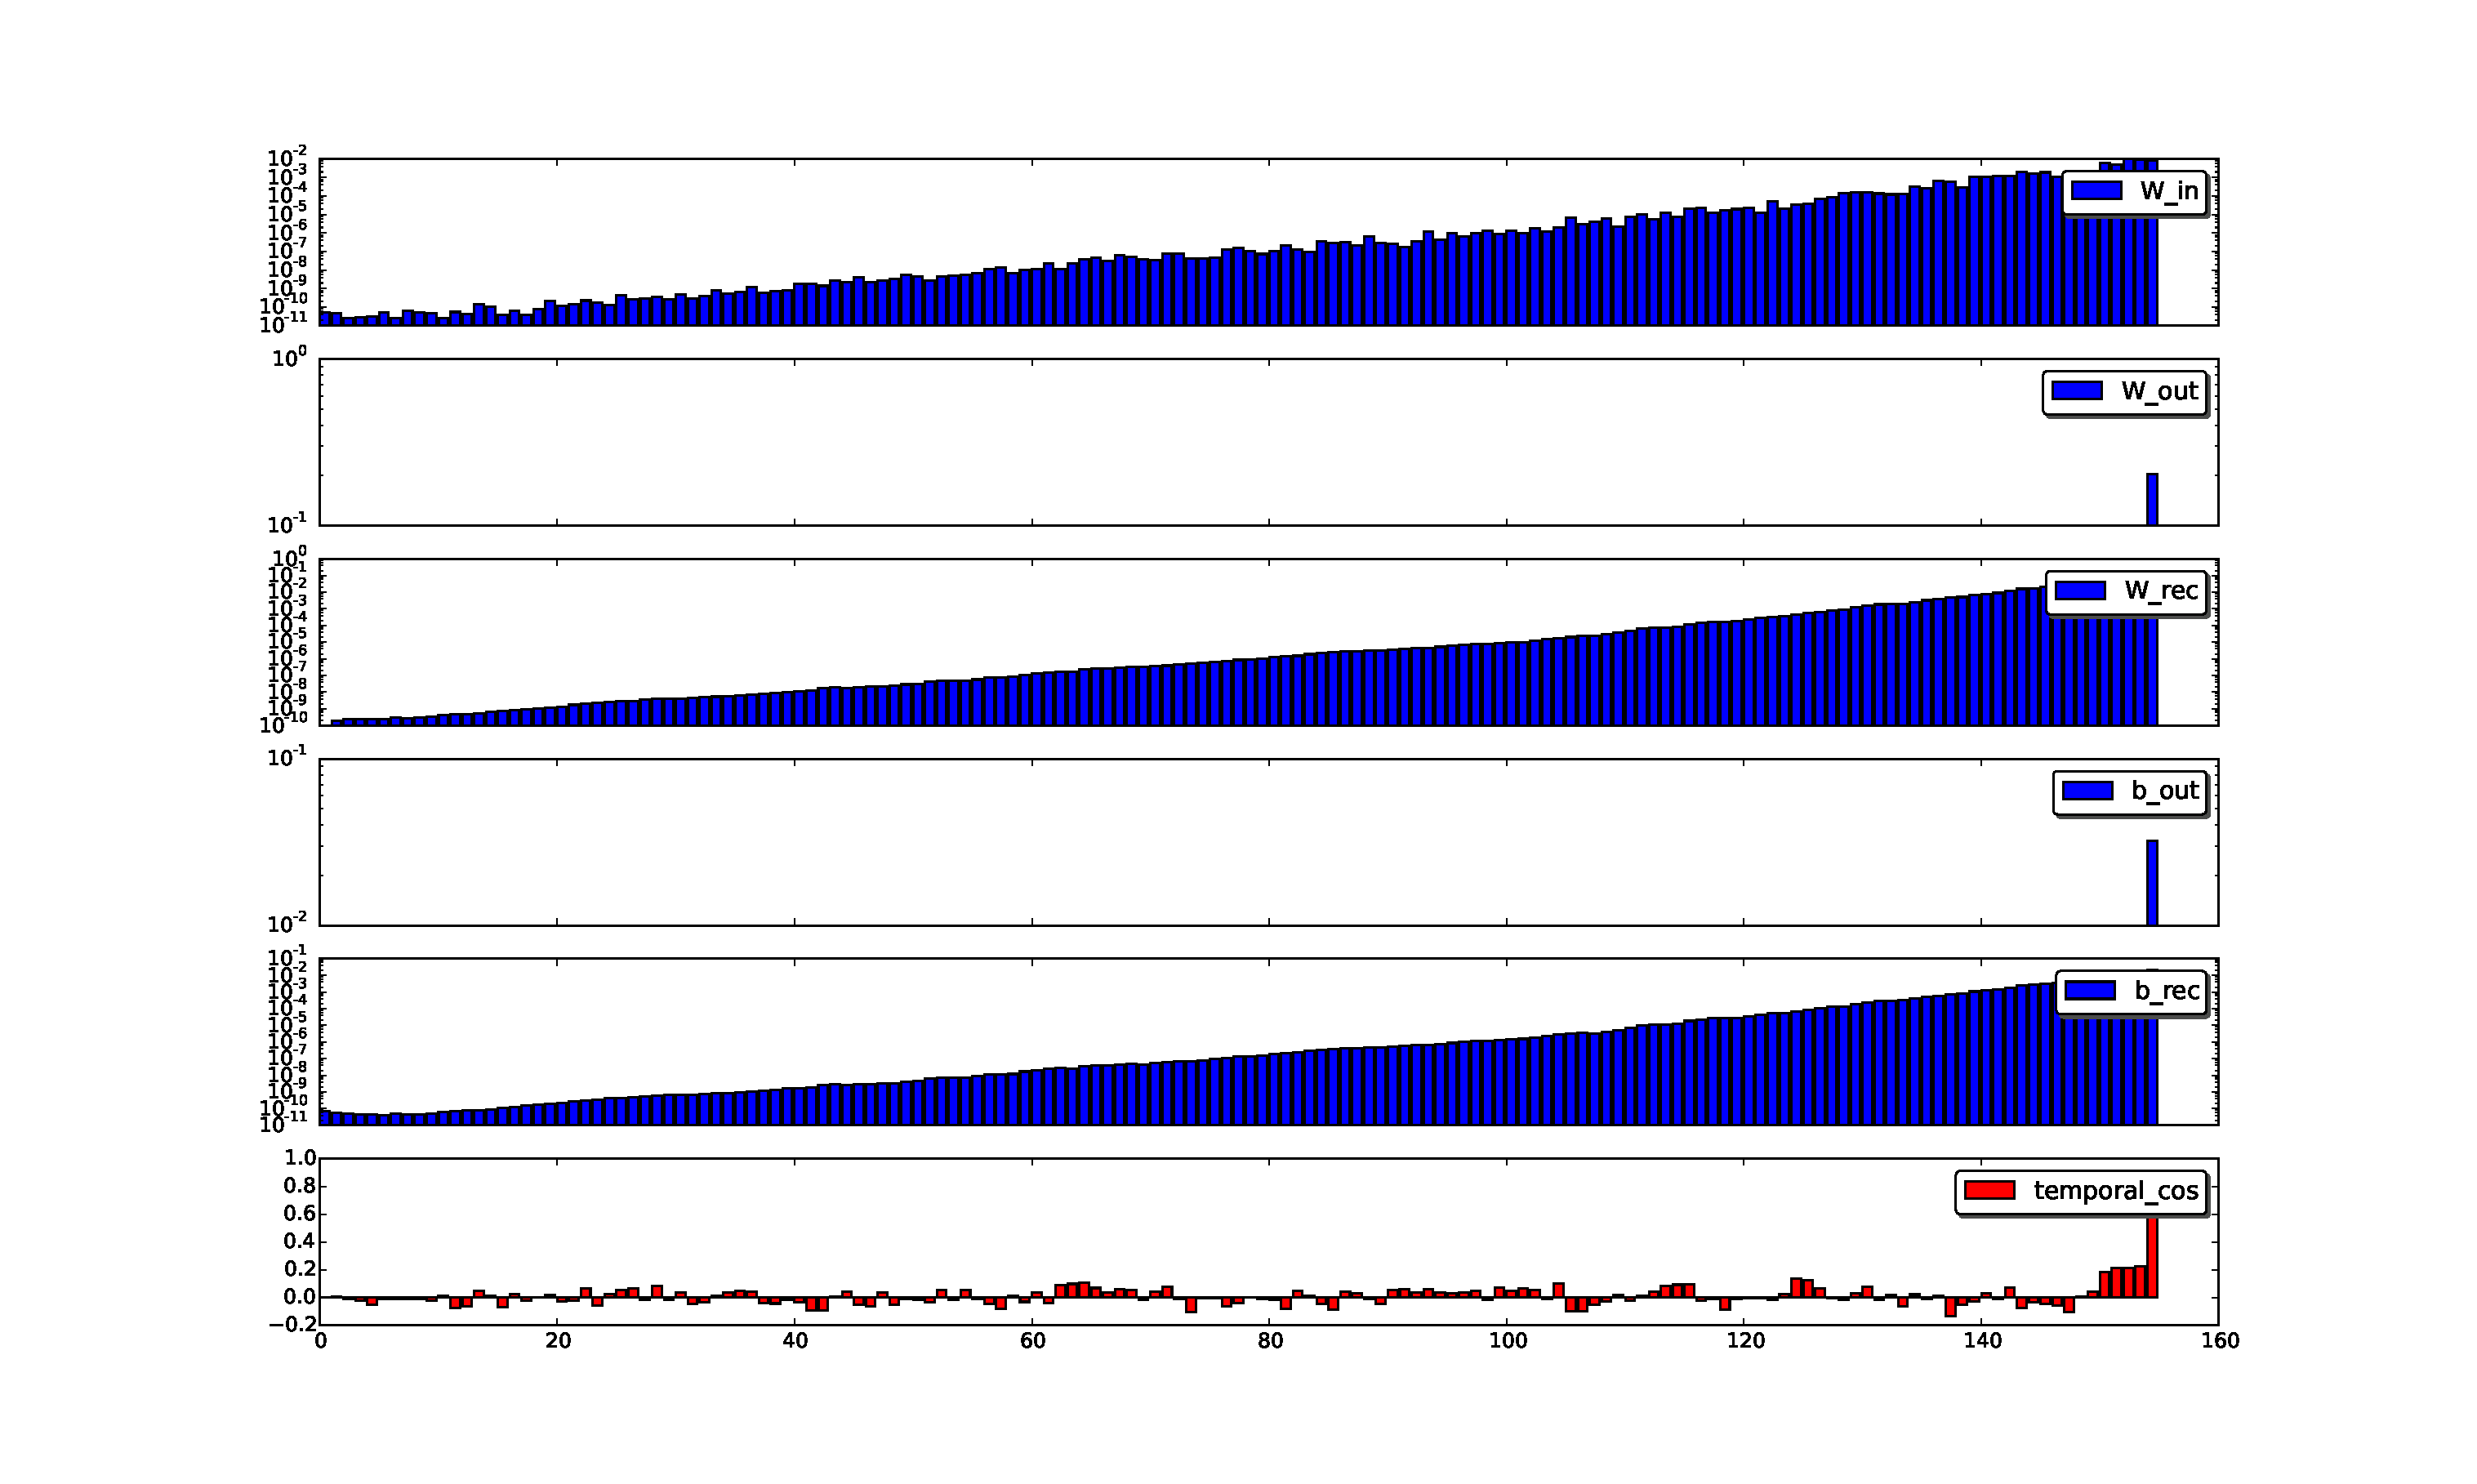
\includegraphics[width=1\textwidth]{temporal_gradients.eps}
\end{figure}
\end{frame}


\section{Solutions}
\begin{frame}{Existent solutions}
	
	\pause
	\begin{itemize}
		\item Long short-term memory (LSTM). Hochreiter, Schmidhuber (1997)
			\begin{itemize}
				\item the network structure is modified with specialized "memory cells"
				\item a truncated version of back-propagation is employed
			\end{itemize}
		\pause
		\item Hessian-Free optimization (HF). Martens (2010)
		\begin{itemize}
			\item a second order method
			\item a "cheap" approximation of the Hessian is employed
			\item the quadratic sub-problem is solved through conjugate gradient + structural damping
		\end{itemize}
		\pause
		\item Pascanu, Bengio (2013)
		\begin{itemize}
			\item a first order method
			\item uses a penalty to deal with the vanishing gradient problem
		\end{itemize}
	\end{itemize}
	
\end{frame}

\begin{frame}{A new proposal}
\begin{itemize}
	\item use the structure of the gradient to compute a descent direction which does not suffer from the vanishing gradient problem
	
	\item normalize the temporal components
	\begin{equation}
	d(\vec{x}) = \sum_{t=1}^T \frac{\nabla L_{|t}(\vec{x})}{\norm{\nabla L_{|t}(\vec{x})}}
	\end{equation}
	
	\item add some randomness for robustness:
		\begin{equation}
		d(\vec{x}) = \sum_{t=1}^T \beta_t\frac{\nabla L_{|t}(\vec{x})}{\norm{\nabla L_{|t}(\vec{x})}},
		\end{equation}
		
		with $\sum_{t=1}^T\beta_t=1, \beta_t>0$
\end{itemize}



\end{frame}

\section{Open issues}
 
\begin{frame}{Open Issues: Initialization}
	
	\begin{itemize}
		\item Some tasks, like the XOR one, are still "unresolved" (even for the other approaches). They cannot be solved with high probability (varying the seed)
		\item it seems to be an \textbf{initialization} matter
	\end{itemize}
	
	Popular strategies for initialization are:
	\begin{itemize}
		\item "small random weights", usually drawn from gaussian or uniform distribution with zero mean. 
		\item sparse initialization: only some weights are actually sampled from a distribution, the other are zero. (Used by HF)
		\item ESN-like initialization
	\end{itemize}
	
\end{frame}

\begin{frame}{Open Issues: Learning rate}
	
	\begin{itemize}	
		\item 	the \textbf{learning rate} is usually tuned by hand, there is no convergence theory for SGD in the non convex case
		\item a \textbf{gradient clipping} technique is often employed:
		\begin{algorithm}[H]
			$\vec{g} \gets \nabla_{\vec{x}} L$\\
			\If{$\norm{\vec{g}} \geq threshold $}{$\vec{g} \gets \frac{threshold}{\norm{\vec{g}}} \vec{g}$}
			\caption{Gradient clipping}
			\label{algo:gradClipping}
		\end{algorithm}
		
		\item  some \textbf{momentum} or \textbf{averaging} technique often yield better convergence time, again tuned by hand
	\end{itemize}
	

\end{frame}

\section{}
\begin{frame}[allowframebreaks]{References}
	\bibliographystyle{ieee}
	\bibliography{biblio}
\end{frame}

\end{document} 
